\chapter{Implementation}

\section{Data set}
% cite it here
For this internship, we used TV broadcasts downloaded from the internet. 
\begin{itemize}
\item The audio files are taken from TV broadcasts. Total duration of audio is around 200 hours.  
\item TV broadcast transcriptions(\textit{closed captions}) of the audio files are provided. The \textit{closed captions} are close to what the audio says, but not exactly the same as the speakers of the audio said.  We call this training set as train.200, containing audio data and the corresponding \textit{closed captions}.
\item 640 million words of TV subtitles are provided. In addition to that, the 640M subtitles are filtered to avoid overlap with the \textit{closed captions} from the TV broadcasts.
\item The development set contains around 8 hours of audio data and their corresponding transcriptions. The transcriptions in the development set are closed to what people said in the audio. 
\end{itemize} 

We prepared two data sets: training set and development set. The training dataset has a total duration of around 200 hours of audio. To evaluate our model, we have a development set. Some metadata are provided in our data, such as: speaker identity of the transcript, genre of the show, date and time of the show, as well as television channel where the show was aired. In addition, each segment has start and end time when the segment was shown in the TV broadcast. All files in full training set have \textit{closed captions}. In contrast, all files in development set have \textit{closed captions} as well as manually annotated human transcription. The transcript is manually and carefully annotated by human. Thus, the transcript is believed to be the closest transcription spoken by speakers in audio files. 

Table \ref{tab:dataset} shows the statistics of the training set and the development set. The second column represents the number of TV shows in each genre; the third column represents the total duration of each genre. Lastly, the forth column(the last column) shows the total duration of speech when the speakers spoke in the audio.
\begin{center}
\label{tab:dataset}
\captionof{table}{Dataset duration}
\begin{tabular}{ | c | c | c | c | c |  }
\hline
No & Data set & \#shows & Duration(h) & Aligned speech (h) \\ \hline
1 & training set & 274 & 193  & 149 \\ \hline
2 & development set & 12 & 8 & 6 \\ \hline
\end{tabular}
\end{center}

 After obtaining about 200 hours of data, a 100 hours subset was created randomly from 200 training set. The 200 hours and 100 hours training set are named as train.200 and train.100 respectively. 

\begin{center}
\captionof{table}{Statistics of train.200 per genre}
\label{statisticstrain200}
\begin{tabular}{ | c | c | c | c|}
\hline
\textbf{Genre} & \textbf{\#shows}  & \textbf{Duration(h)} & Aligned speech(h) \\ \hline \hline
advice & 40 & 26 & 22 \\ \hline
children & 51 & 19 & 14 \\ \hline
comedy & 19 & 8 & 6 \\ \hline
competition & 30 & 21 & 16 \\ \hline
documentary & 29 & 22 & 14 \\ \hline
drama & 20 & 14 & 10 \\ \hline
events & 24 & 38 & 29 \\ \hline
news & 61 & 42 & 37 \\ \hline
\end{tabular}
\end{center}

Table \ref{statisticstrain200} shows that the statistics of our training data. Our data has 8 genres. The second column(from left) shows the number of shows corresponding to their genre; the third columns shows the total audio duration of each genre; the forth column shows the total speech duration. The data with the news genre and events genre  have the most duration and the second most duration respectively. In contrast, the comedy genre data have the least duration.

%Table \ref{statisticstrain200} shows the statistics of each genre in the train.200 training set. 

\section{Experimental setup}
In this section, we explained how we did the experiments. We elaborated how to build language models,   the acoustic model, and  how to decode the data set for the data selection and the model evaluation.

\subsection{Language model}
\subsubsection{Library: SRILM}
SRILM is a toolkit  written in C++, for developing statistical language models for speech recognition and other natural language applications \cite{Stolcke02srilm}. SRILM allows creating a language model from a text corpus, interpolating several language models, pruning a language model, and estimating the perplexity of a language model using  test corpus. 

The code bellow is an example how to make a 4-gram language model with input from $CORPUS$ and interpolated with Kneser-ney interpolation \cite{KneserNey1993}. The syntax is pretty straightforward and easy to understand. The resulted language model will be written in arpa language model format.
\begin{verbatim}
ngram-count -order 4 -kndiscount -interpolate -sort -text CORPUS -lm LM
\end{verbatim}

\subsubsection{Implementation}
\label{3LM}
This internship experimented with three different kinds of language model for speech recognition. All language models are based on four gram language model. 

\begin{enumerate}
\item LM.200 \\
This language model, named as LM.200, was produced from the \textit{closed captions} of 200 hours training set(train.200).   LM.200 was used for the baseline speech recognizer to select the "good" subset of data.  Table \ref{statsTrain200} displays the statistics of the language model. The closed caption dataset has 33,914 words. Section \ref{ch3:dataselection} mentions the more constrained language model for the data selection pipeline. In the internship, we utilized LM.200 as the more constrained language model.

\begin{center}
\captionof{table}{Statistics of LM.200}
\label{statsTrain200}
\begin{tabular}{ | c | c | c | }
\hline
\textbf{No.} & \textbf{File}  & \textbf{Information} \\ \hline \hline
1 & word.200 & 33,914 words \\  \hline
2 & LM.200 & uni-gram=33916 \\ 
 & & bi-gram=402299 \\ 
& & tri-gram=111868 \\  
& & 4-gram=64801 \\  \hline
\end{tabular}
\end{center}

\item LM.7weeks+subtitles.limited.1e-9 \\
A language model was generated from the \textit{closed captions} of 1600 hours transcription(7weeks TV broadcast \textit{closed captions}) and interpolated with a language model from the big TV subtitles with ratio 0.9/0.1. The ratio means that estimation of language model of \textit{closed captions} is multiplied by 0.9, the estimation of big subtitle language model is multiplied by 0.1, and and they are summed together. The language model was limited by top 160,000 frequent word list and pruned by $10^{-9}$ resulting in LM.7weeks+subtitles.limited.1e-9.   Section \ref{ch3:dataselection} mentions the less constrained language model for the evaluation pipeline. In the internship, we utilized  LM.7weeks+subtitles.limited.1e-9  as the less constrained language model.



\begin{center}
\begin{tabular}{ | c | c | c | }
\hline
\textbf{No.} & \textbf{File}  & \textbf{Information} \\ \hline \hline
1 & word.160k & 160,000 words \\  \hline
2 & LM.7weeks & ngram 1=91836 \\
 & & ngram 2=1817881 \\
 & & ngram 3=980925 \\
 & & ngram 4=847736 \\  \hline
3 & LM.subtitles & ngram 1=756644 \\
 & & ngram 2=27144330 \\
 & & ngram 3=37162518 \\
 & & ngram 4=57912280 \\ \hline
4 & LM.7weeks+subtitles & ngram 1=768522 \\
 & & ngram 2=27441072 \\
 & & ngram 3=37312673 \\
 & & ngram 4=58183256 \\ \hline
5 & LM.7weeks+subtitles.limited & ngram 1=160002 \\
 & & ngram 2=24926818 \\
 & & ngram 3=32102763 \\
 & & ngram 4=44253079 \\ \hline
5 & LM.7weeks+subtitles.limited.1e-9 &ngram  1= 160002 \\
 & & ngram  2=   5251197 \\
 & & ngram  3=   3876171 \\
 & & ngram  4=   2453067 \\ \hline
\end{tabular}
\end{center}

\item LM.genres \\
Eight language models were generated from each genre(LM.documentary, LM.news, LM.events, LM.drama, LM.competition, LM.comedy, LM.children, and LM.advice). Then, each language model was interpolated with the big subtitle LM with  ratio 0.9/0.1, limited by the top 160,000 word list, and pruned by $10^{-9}$ threshold. The language model was used in the new proposed data selection only. To build language models, we utilized SRILM.

\begin{center}
\begin{tabular}{ | c | c | c | }
\hline
\textbf{No.} & \textbf{File}  & \textbf{Information} \\ \hline \hline
1 & LM.documentary & ngram 1=37542
ngram 2=437631
ngram 3=135632 \\
& & ngram 4=90381   \\ \hline
2 & LM.news & ngram 1=44588
ngram 2=661625
ngram 3=305473 \\
& & ngram 4=255125  \\ \hline
3 & LM.events & ngram 1=23717
ngram 2=306938
ngram 3=125934 \\
& & ngram 4=95203  \\ \hline
4 & LM.drama & ngram 1=21345
ngram 2=202078
ngram 3=60920 \\
& & ngram 4=40073  \\ \hline
5 & LM.competition &  ngram 1=33269
ngram 2=385257
ngram 3=124584 \\
& & ngram 4=89642 \\ \hline
6 & LM.comedy & ngram 1=20180
ngram 2=165073
ngram 3=39353 \\
& & ngram 4=23877  \\ \hline
7 & LM.children &  ngram 1=27029
ngram 2=287141
ngram 3=84063 \\
& & ngram 4=57851 \\ \hline
8 & LM.advice & ngram 1=30545
ngram 2=397766
ngram 3=154416 \\
& & ngram 4=108794  \\ \hline
\end{tabular}
\end{center}

\end{enumerate}




\subsection{Acoustic model}
\subsubsection{Library: Kaldi}
Kaldi is a toolkit, written in C++, which comprises several tools to experiment and build a speech recognition system \cite{PoveyASRU2011}. Kaldi supports several operations to build a speech recognition system, such as: extracting feature vectors, acoustic modeling, training acoustic models, and creating decoding graph as well as decoding audio inputs into lattices. Kaldi provides several features, such as:
\begin{itemize}
\item It supports finite state transducer(FST), which is based on OpenFST library. The FST is used to build a decoding graph with the inputs of acoustic model, language model, and lexicon.
\item It is extensible and provides complete recipes. Kaldi gives many recipes to build acoustic model, such as: gaussian mixture model, deep neural network, etc.
\end{itemize}

\subsubsection{Acoustic model implementation}
%GMM
%Before training the DNN acoustic model, GMM-HMM must be trained first. GMM-HMM is able to perform force alignment on the flat start(without phoneme-to-audio alignment). The labeling of each acoustic input is compulsory to train the TDNN acoustic model. 

We utilized TED-LIUM's recipe(nnet3 in Kaldi) to train the TDNN acoustic model. The feature vectors are MFCC, consisting of 40 feature values. The TDNN architecture has 6 hidden layers, where each hidden unit  utilizes rectified linear unit(RELU) activation function. The TDNN outputs around 9000 output nodes with softmax activation function. Moreover, the TDNN architecture is implemented by leveraging the subsampling technique. Table shows the parameters and subsampling splice configuration we used in the architecture.

\begin{center}
\captionof{table}{Parameters of  theTDNN acoustic model}
\label{TDNNparams}
\begin{tabular}{ | c | c | }
\hline
\textbf{Parameter} & \textbf{Method}  \\  \hline \hline
initial learning rate & 0.0015 \\
final learning rate & 0.00015 \\ \hline
mini batch size & 512 \\ \hline
epoch & 3 \\ \hline
subsampling splice & \\
layer 1 & $t-2,t-1,t,t+1,t+2$ \\
layer 2 & $t-1,t+2$ \\
layer 3 & $t-3,t+3$ \\
layer 4 & $t-7,t+2$ \\
layer 5 & $t-3,t+3$ \\
layer 6 & $t$ \\  \hline
\end{tabular}
\end{center}
% features
% architecture

% hyperparameters
% -splice
% -learning rate
% -training

\subsection{Recognition}
After training the acoustic models and building the language models, we recognize a data set. The recognition is useful for data selection(computing the new word error rate as well as phone error rate ) and evaluate how good our data selection is. In overall, the recognition(or decoding) process works as following:
\begin{enumerate}
\item Create a decoding graph from the acoustic model, the language model, and the lexicon. In Kaldi's implementation, it transforms the  acoustic model, the language model, and the lexicon into a weighted finite state transducer(WFST).
\item Decode the dataset using the WFST. In Kaldi, the decoding process will result in a lattice. Lattice is a decoding graph which represents some variants of the recognition. Providing only one best recognition is not practical; thus lattice is the way to represent the recognition/decoding result. 
\item Compute the best path of words or phones in the lattice and calculate the WER as well as PER. Kaldi produces two ctm files(word and phone ctm files) which are the best decoding results which the algorithm can obtain. The ctm file consists of words(or phone) in the transcription with its start and end times relative to the audio. 

Sclite is a tool for evaluating and scoring the output of speech recognition systems. By utilizing sclite, the ctm file(the hypothesized word/phone from the ASR) is compared with the transcriptions(the \textit{closed captions} or the detailed transcription) and the error rate is calculated.  
\end{enumerate}

\subsubsection{Data Selection}
To select the good data for the next iteration, we need to re-recognize the training set and calculate the new value of matched word phone matched error rate, and average word duration. Here are the steps for computing the value of PMER and WMER:
\begin{enumerate}
\item Recognize the training set with the trained acoustic model, the language model, and the lexicon. This will result new decoding transcriptions.
\item By utilizing sclite, we can compare the \textit{closed captions} and decoding transcriptions. After comparing, sclite automatically generates the numbers of correct words, insertions, deletions, and substitutions which is written in a file with extension ".prf". Figure \ref{prf} illustrates a segment with its corresponding \textit{closed caption} and decoding transcription.  REF represents the closed caption, while HYP represents the decoding transcription. After knowing the number of correct words, insertions, deletions, and substitutions, the values of PMER, WMER, and AWD can be computed.

\begin{figure}[H]
\caption{The example}
\label{prf}
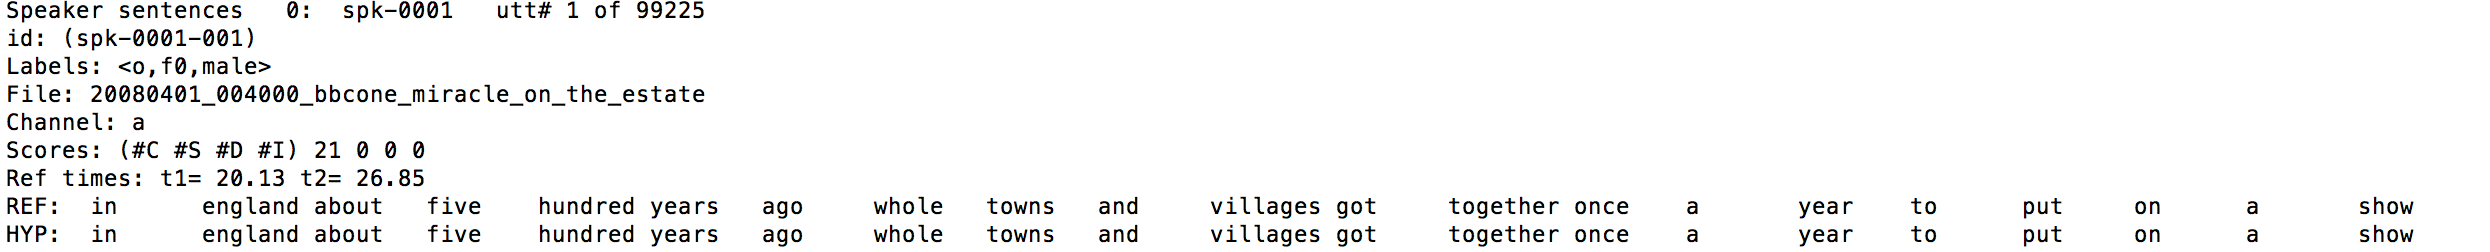
\includegraphics[scale=0.5]{prf} 
\centering
\end{figure}

\item After computing the new value of PMER, WMER, and AWD for each segment, we select segments with AWD in the range of $0.165 \leq AWD \leq 0.66$ and then sort the selected data based on PMER. We only choose top 100 hours data which has the lowest PMER.

\end{enumerate} 



\subsubsection{Evaluation}
To evaluate how good our data selection is, we need to evaluate the automatic speech recognizer. In every data selection iteration, we train an acoustic model, build a speech recognizer (with the acoustic model, the language model(LM.7weeks+subtitles.limited.1e-9), as well as the lexicon),  and recognize the development set. After decoding and computing WER of development set, we compare the WER with the previous iteration. If the new WER is lower, we can continue the iteration; otherwise, stop the iteration. 

%\subsubsection{Experiments}

\section{Experiment resources}
To run our experiment, we utilized grid 5000 server cluster. Grid 5000 is a computing cluster with a focus on parallel and distributed computing \cite{Grid5000}. It has several key features:
\begin{itemize}
\item It provides a large amount of resources, over 1000 nodes, and massive volume of hard disk.
\item The experiment is highly configurable where we can specify number of nodes and the criteria of the nodes which we will use.
\item We can do advanced monitoring of memory usage, cpu usage, and the log of our experiment which later be used to analyze the experiment.
\end{itemize}

The following is the description of resources which we leveraged for this internship based on the tasks:
\begin{enumerate}
\item Train acoustic models: 1 computer with GPU and 8 computers without GPU. At least one computer with GPU is compulsory because we can harness GPU to parallelization the computation of DNN training. 
\item Create decoding graph only needs one computer because the Kaldi recipe does not need parallelization for this process.
\item Decoding the ASR leverages 20 computers. Usually one computer can recognize one hour of audio within one hour. Therefore, the more computer we use, the faster the decoding process will be. 
\item The error rate computation and data selection process only utilizes one computer. 
\end{enumerate}
% server
% exectution time

